\section{ГОСТ Р 34.11-94}\index{хеш-функция!ГОСТ Р 34.11-94|(}
\selectlanguage{russian}

Устаревший российский стандарт ГОСТ~Р~34.11-94~\cite{GOST-94} <<Информационная технология. Криптографическая защита информации. Функция хэширования>> описывает хеш-функцию, которая в целом также построена с использованием структуры Меркла~---~Дамгора\index{структура!Меркла~---~Дамгора}, но со своими особенностями (рис.~\ref{fig:gost-94}).

\begin{figure}[htb]
    \centering
    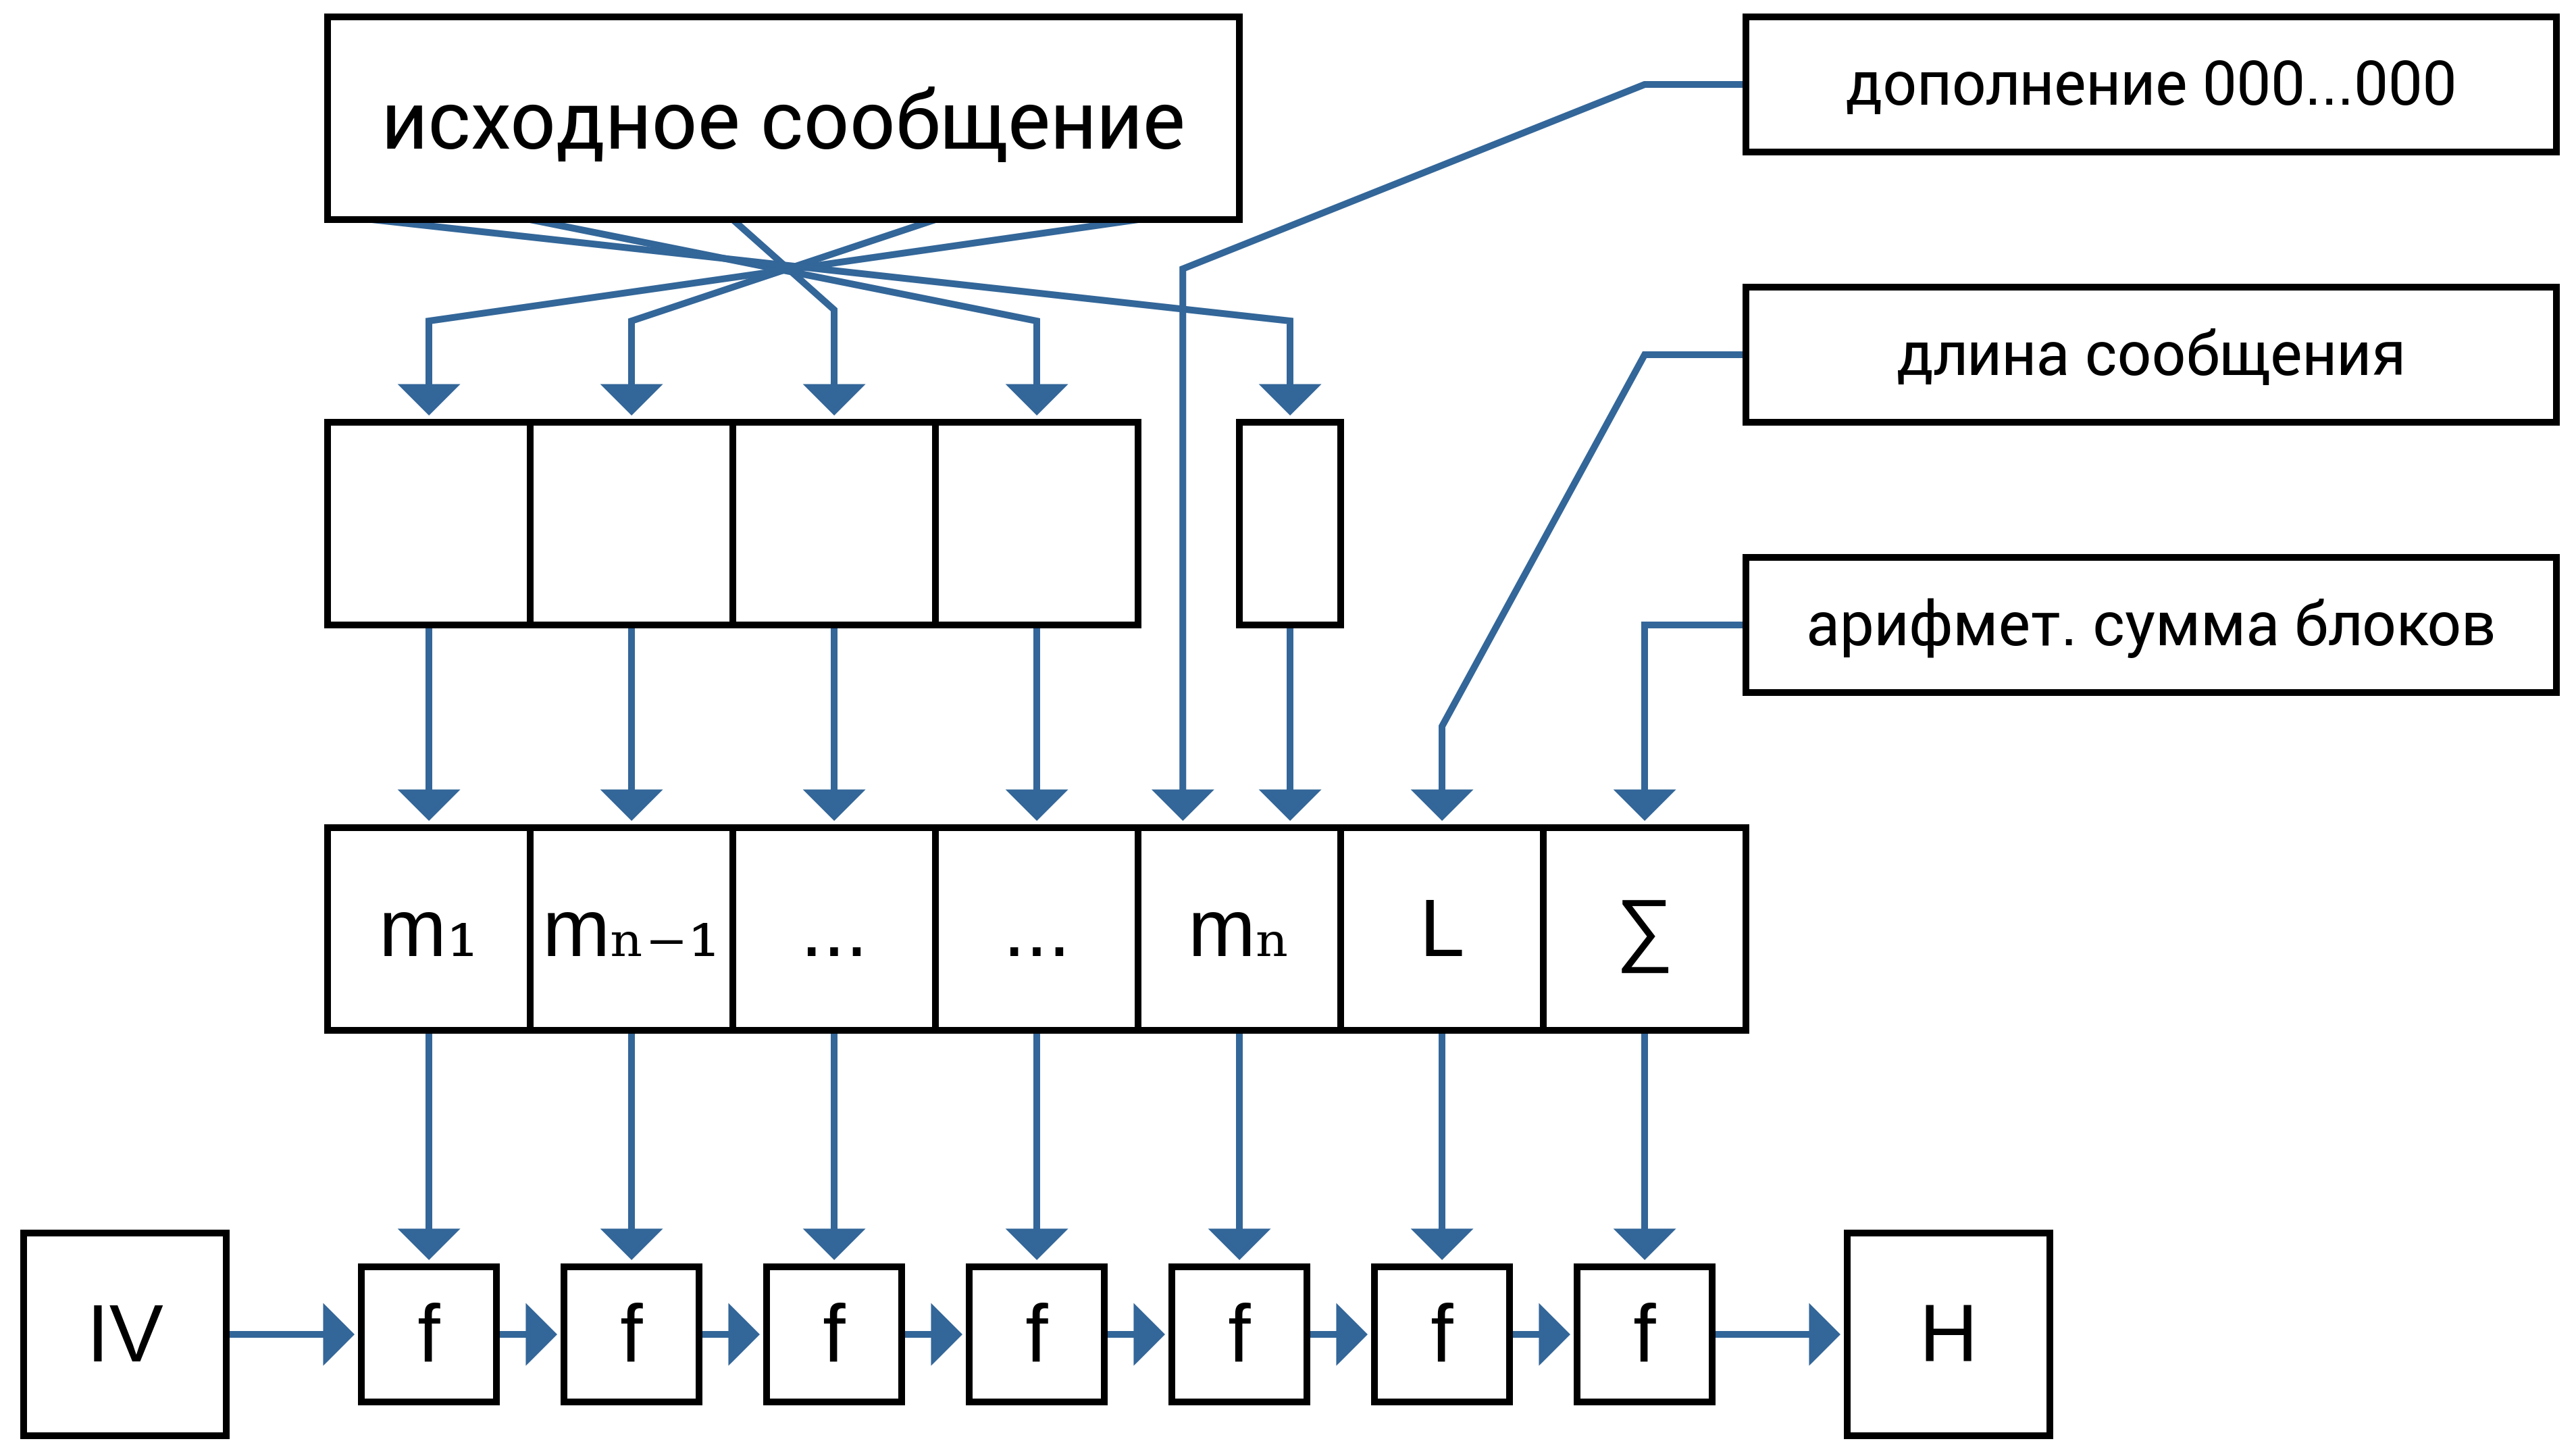
\includegraphics[width=\textwidth]{pic/gost-94}
    \caption{Структура хеш-функции ГОСТ~Р~34.11-94}
    \label{fig:gost-94}
\end{figure}

\begin{itemize}
  \item Сообщение обрабатывается не с начального блока, а с конечного. Для целей удобства записи считается, что исходное сообщение разбивается на блоки\[
  M = m_n \| m_{n-1} \| \dots \| m_2 \| m_1.
\]
  \item Дополнение происходит в блоке $m_n$, то есть в последнем обрабатываемом, но первом с точки зрения исходного текста. Блок дополняется нулями <<слева>> (то есть перед открытым текстом) до размера в 256 бит.
  \item В отличие от хеш-функции MD5\index{хеш-функция!MD5} присутствует финальное преобразование, которое выполняется над арифметической суммой всех обработанных блоков. В будущем аналогичное преобразование будет использоваться и в хеш-функции ГОСТ~Р~34.11-2012 <<Стрибог>>\index{хеш-функция!Стрибог|(}.
  \item Для хеш-функции не определены стартовый вектор $H_0 = IV$, внутренние параметры раундовой функции компресии (параметры $s$-блоков используемой функции шифрования) и способ представления результатов хеширования в виде 16-ричной и/или Base64-записи, что привело к появлению нескольких, несовместимых между собой реализаций алгоритма.
\end{itemize}

\begin{figure}[htb]
    \centering
    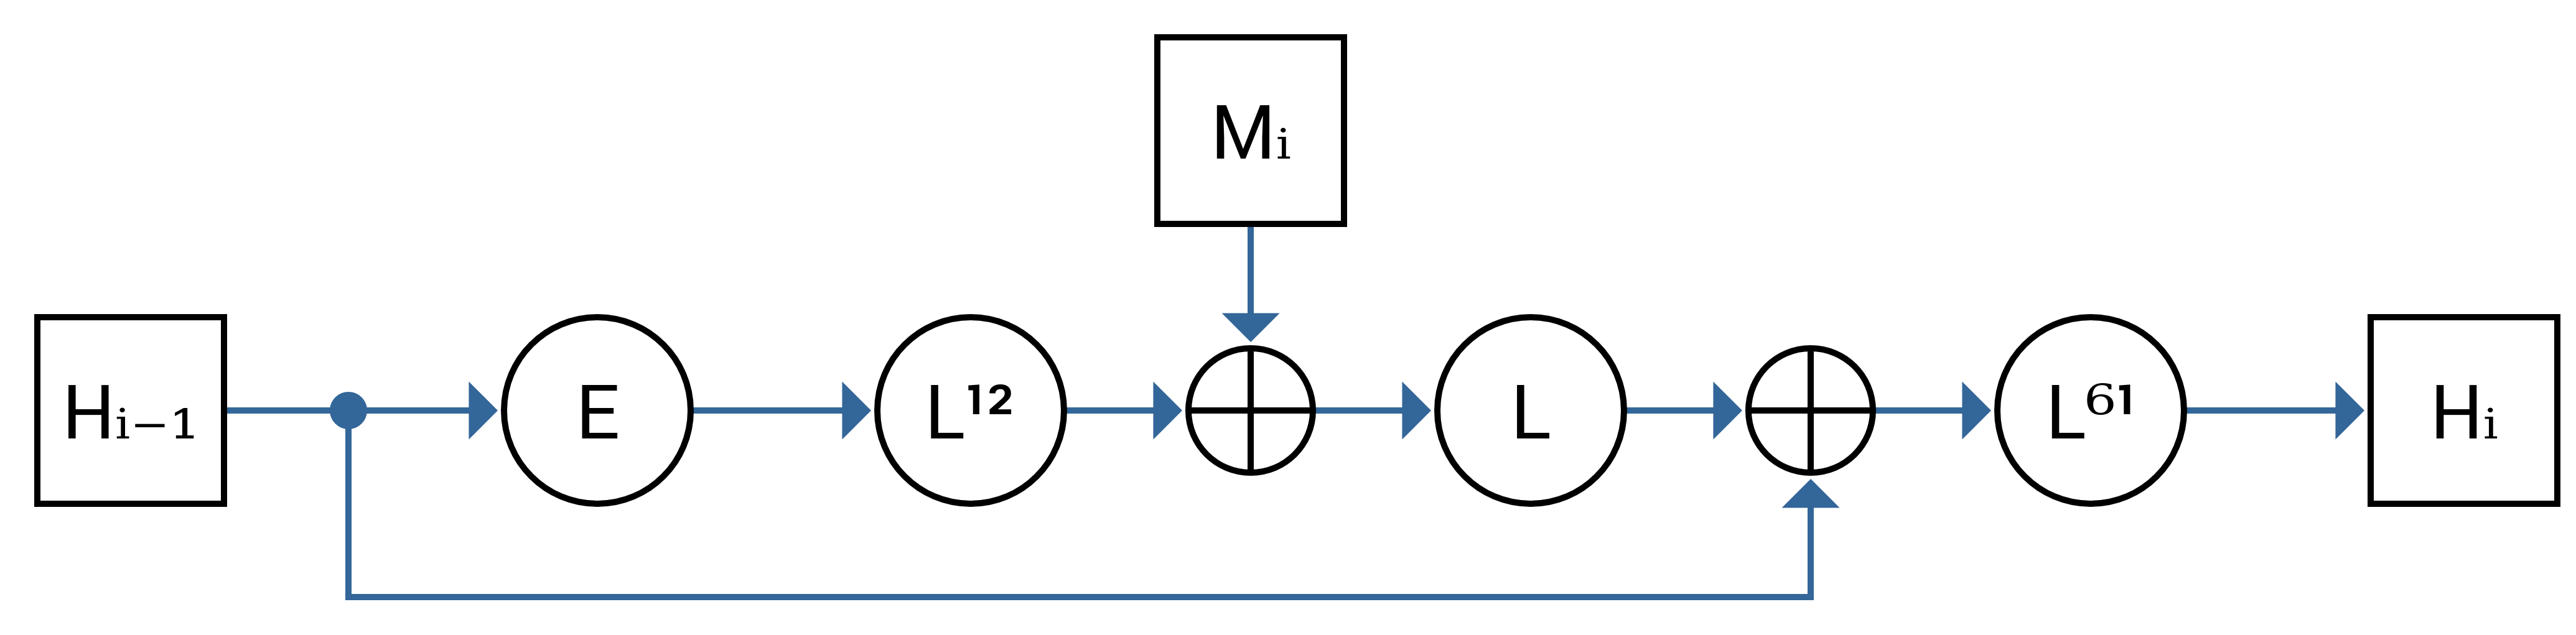
\includegraphics[width=\textwidth]{pic/gost-94-elxlxl}
    \caption{Последовательность преобразований в раундовой функции сжатия ГОСТ~Р~34.11-94}
    \label{fig:gost-94-elxlxl}
\end{figure}

Раундовая функция сжатия состоит из нескольких последовательных преобразований, как показано на рис.~\ref{fig:gost-94-elxlxl}.

\begin{figure}[htb]
    \centering
    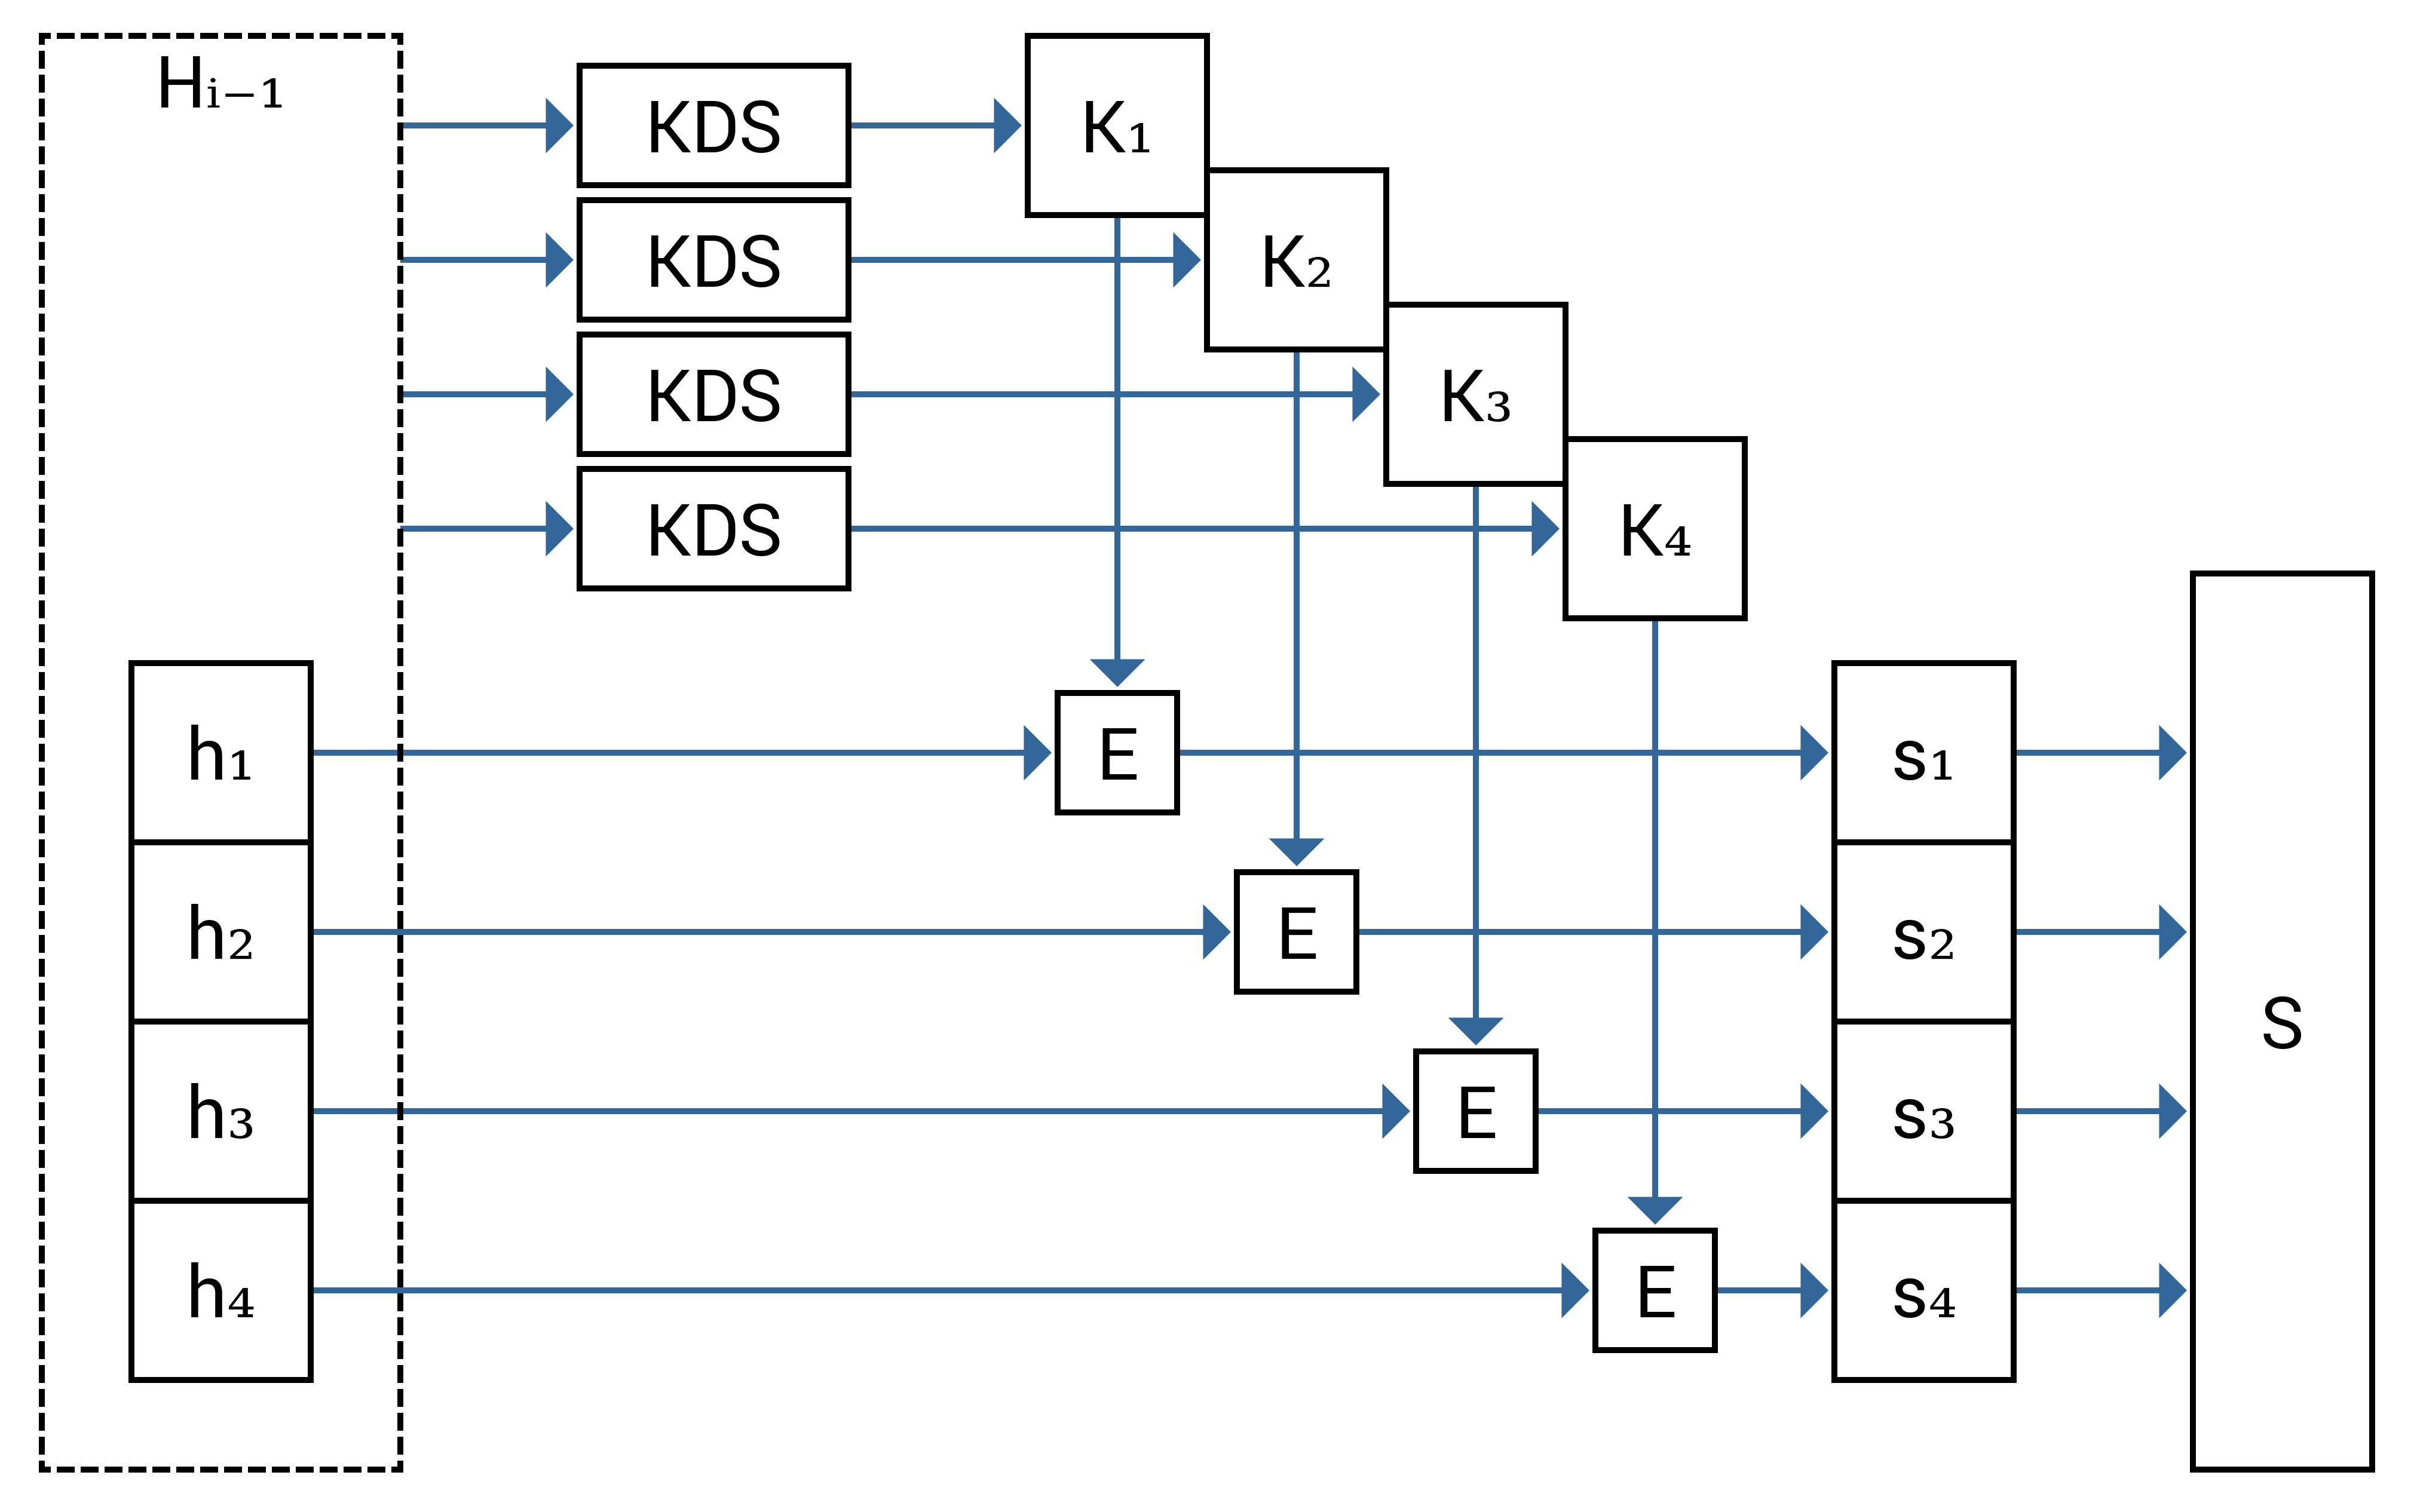
\includegraphics[width=0.75\textwidth]{pic/gost-94-encrypt}
    \caption{Шифрующее преобразование $E$ в раундовой функции сжатия хеш-функции ГОСТ~Р~34.11-94}
    \label{fig:gost-94-encrypt}
\end{figure}

\begin{itemize}
  \item Результат обработки предыдущего блока $H_{i-1}$ разделяется на 4 части.  Каждая из них шифруется собственным ключом (также полученным из $H_{i-1}$) с помощью блочного шифра ГОСТ~28147—89 в режиме простой замены, как показано на рис.~\ref{fig:gost-94-encrypt}. Результат шифрования конкатенируется (в $S$).

\begin{figure}[htb]
    \centering
    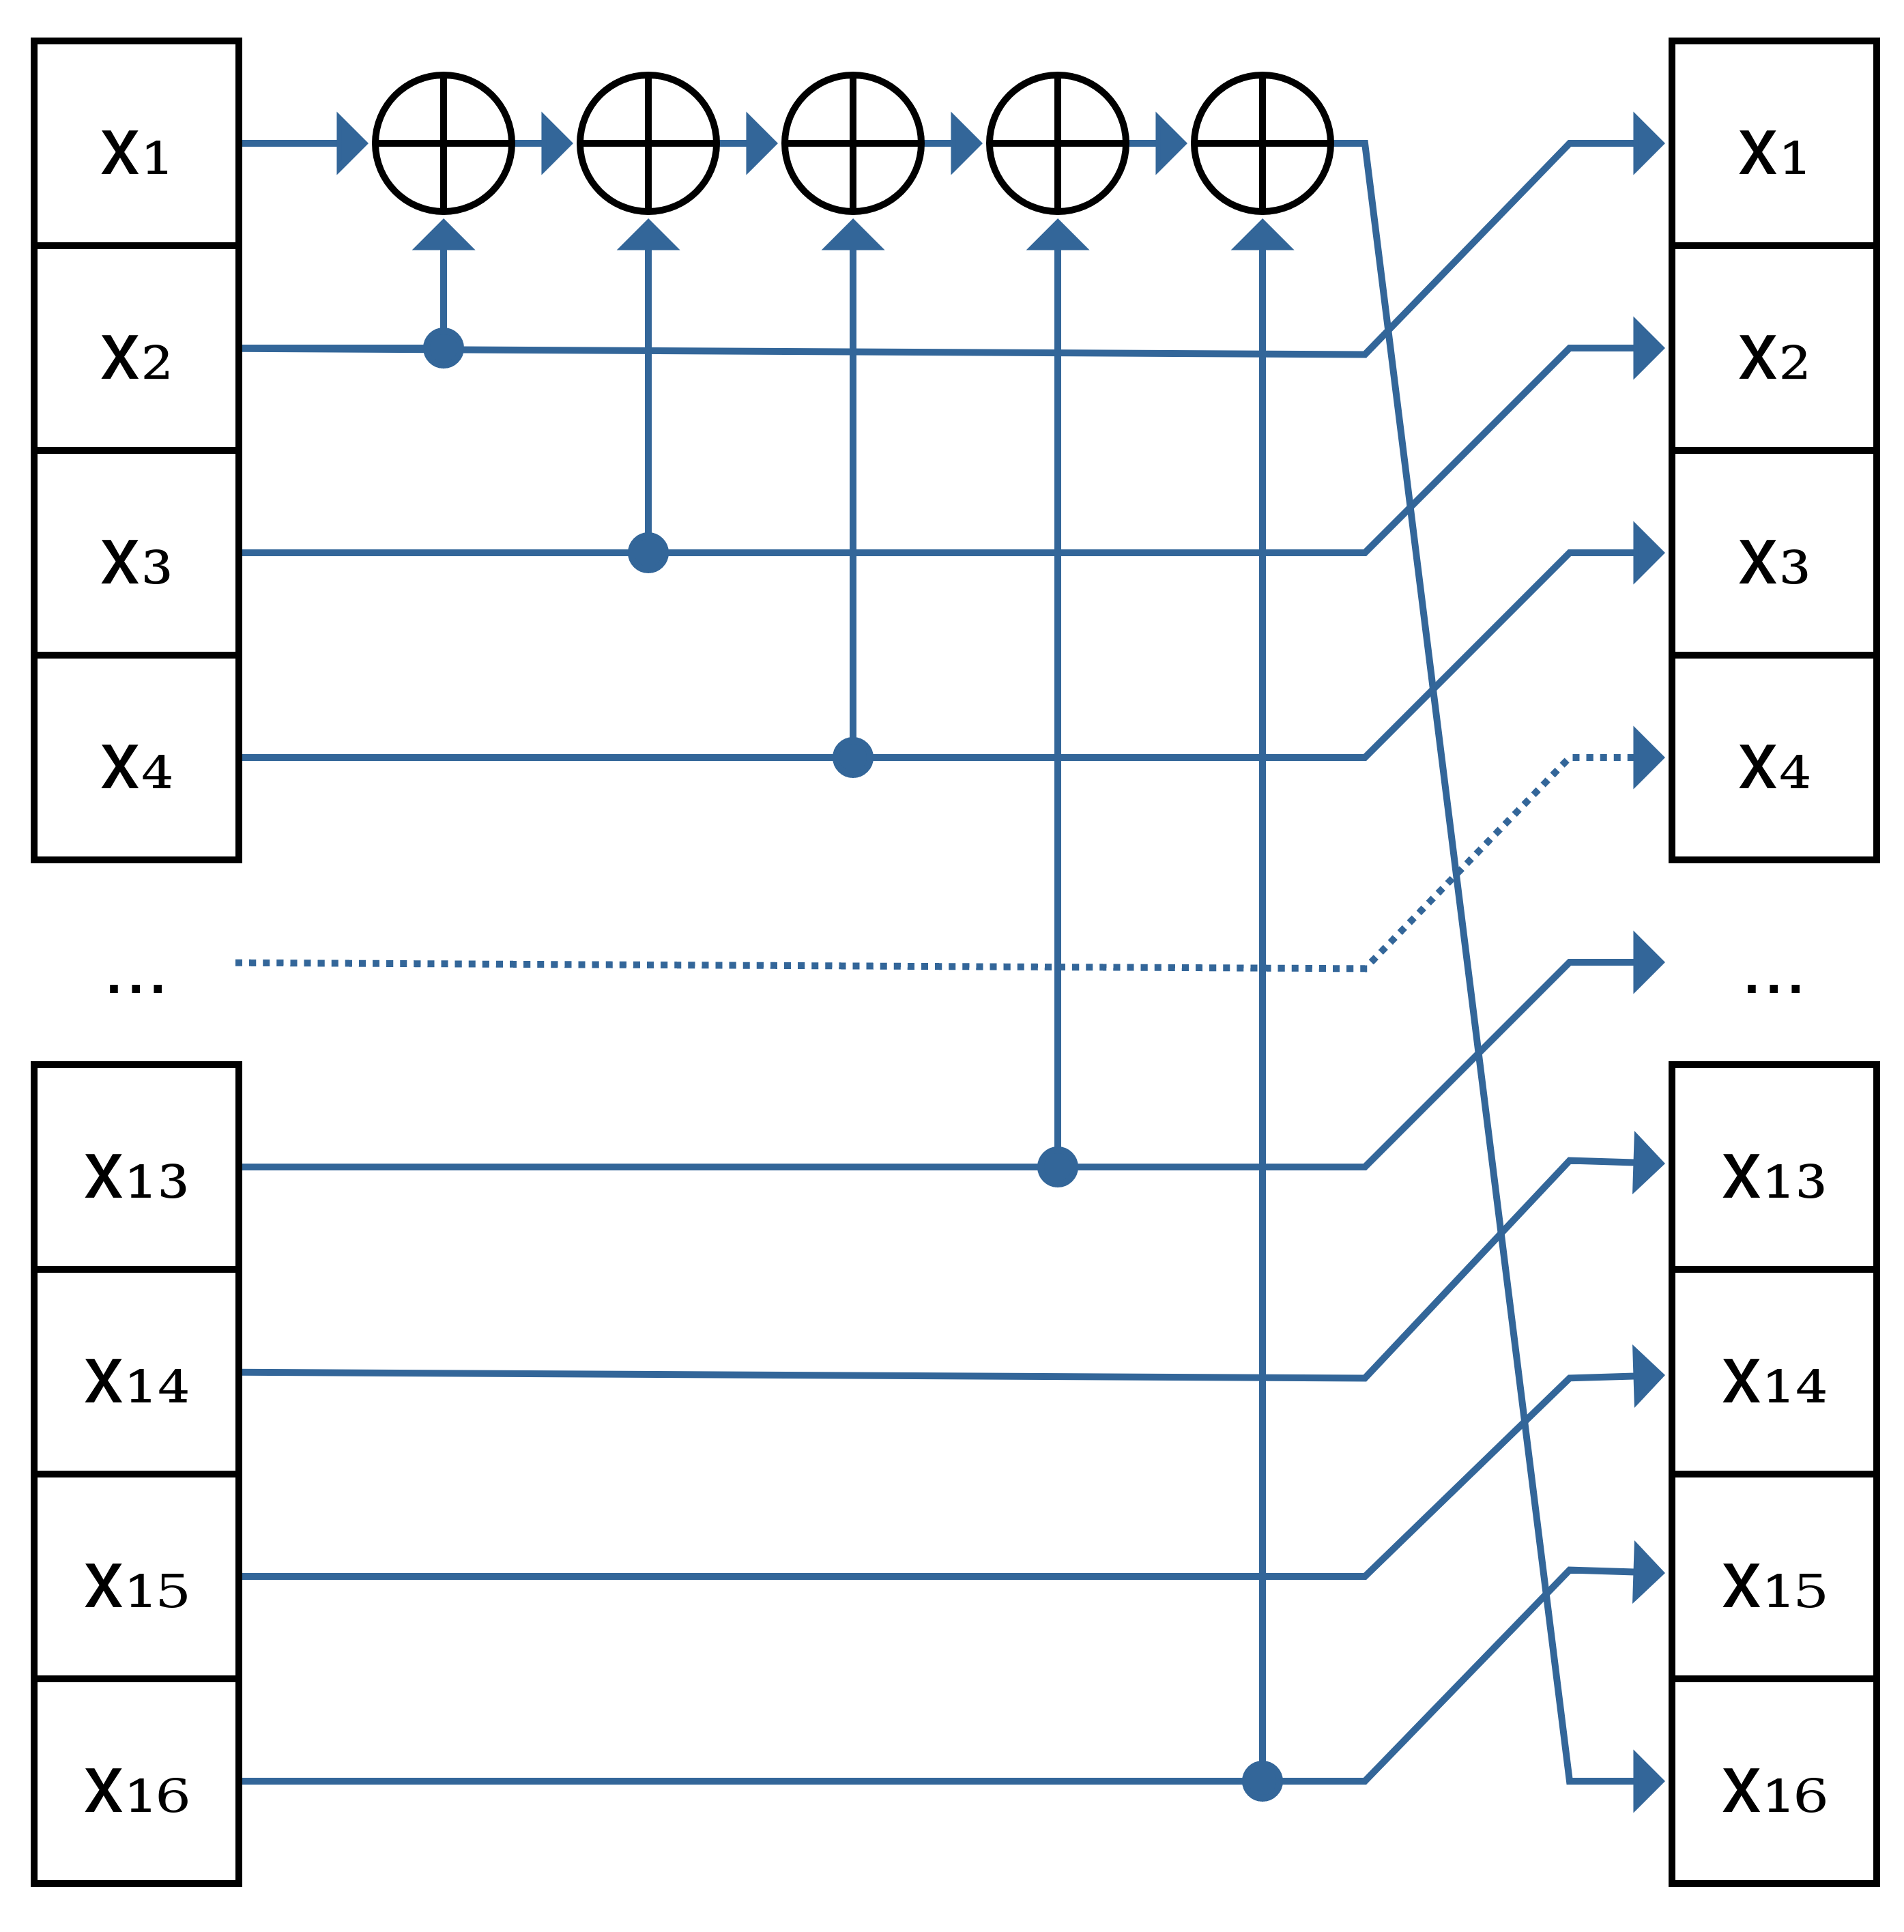
\includegraphics[width=0.55\textwidth]{pic/gost-94-permutation}
    \caption{Линейное преобразование $L$ в раундовой функции сжатия хеш-функции ГОСТ~Р~34.11-94}
    \label{fig:gost-94-permutation}
\end{figure}

  \item Блок $S$ разбивается на 16 частей (по 16 бит), далее производится линейное преобразование, изображённое на рис.~\ref{fig:gost-94-permutation}. Все блоки кроме $x_1$ сдвигаются на одну позицию вправо. Значение первого блока $x_1$ складывается побитово по модулю 2 (операция XOR) со значениями блоков $x_2, x_3, x_4, x_13$ и $x_15$, результат помещается в блок $x_16$. Данное преобразование ($L$) повторяется 12 раз. 
  \item К результату предыдущих преобразований складывается побитово по модулю 2 (операция XOR) с обрабатываемым блоком $m_i$. Это первый и единственный раз, когда в преобразованиях участвует обрабатываемая последовательность. Результат сложения пропускается через линейное преобразование $L$ 1 раз.
  \item К результату побитово по модулю 2 (операция XOR) добавляется результат обработки предыдущей раундовой функции сжатия $H_{i-1}$. Результат сложения пропускается через линейное преобразование $L$ 61 раз.
\end{itemize}

В 2008 году криптоаналитики из Европы сумели уменьшить количество операций для поиска коллизий в $2^{23}$ раза (по сравнению с ожидаемым количеством $2^{128}$, \cite{Boldyreva:Fehr:ONeill:2008}). Хотя в целом это не позволяет говорить о криптографической ненадёжности хеш-функции на текущий момент, но показывает, что при её проектировании были допущеные определённые ошибки. С 1 января 2013 года на территории России стандарт был заменён на ГОСТ Р 34.11-2012 <<Стрибог>>.

\index{хеш-функция!ГОСТ Р 34.11-94|)}
